\section{Problemstellung}
Wie in der Einleitung bereits angemerkt, beschreibt \glqq Information Retrieval\grqq das Bereitstellen spezieller Informationen aus einer meist großen, unsortierten Datenmenge. Dabei bekommt das System eine vom Nutzer gestellte Query (Abfrage) und versucht auf dessen Basis, Daten, die meist als Dokumente vorliegen, zurückzuliefern.
Im Gegensatz zu Abfragen im Datenbankumfeld beinhaltet die Query jedoch keinerlei Informationen, um ein spezielles Element eindeutig identifizieren zu können. Dies soll ein IR-System auch nicht leisten. Vielmehr sollen Ergebnisse zurückgeliefert werden, die mit hoher Wahrscheinlichkeit Relevanz bzgl. der gestellten Query besitzen. Der Nutzer selektiert dann die für diesen nötigen Dokumente.
\newline
Mathematisch lässt sich dies folgendermaßen formulieren:
Aus einer Dokumentenmenge $D$ soll mithilfe einer Funktion eine Teilmenge $D_1$ von $D$ ermittelt werden, die relevant für eine Abfrage $q$ ist.
\newline
Um diese Funktion sinnvoll definieren zu können, muss jedoch zuvor die Menge aller Queries, sowie die Menge aller Tokens definiert werden:
\begin{defi}
	Sei $d$ \in $D$ ein Dokument. Die Menge $T_d$ ist nun die Menge aller Wörter, die in dem Dokument $d$ enthalten sind: $T_d$ = $\{$$t_1$, .., $t_n$$\}$.
	\newline
	Die Menge $T$ ist die Menge aller Terme, die in den Dokumenten aus $D$ vorkommen, also:
	$T$ = $T_{d1}$ \cup .. \cup $T_{dn}$ mit $d_i$ \in $D$.
\end{defi}

\begin{defi}
	Mithilfe der letzten Definition kann nun die Menge aller möglichen Queries definiert werden:
	$Q$ \subseteq $2^T$
\end{defi}

\begin{defi}
	Eine Funktion $f$: $Q$ \rightarrow $D_1$ heißt Retrievalfunktion, wobei $D_1$ \subseteq $D$ gilt und $Q$ die Menge aller Queries ist.
\end{defi}

Nachdem die Problemstellung formuliert ist, muss eine Strategie entwickelt werden, wie die Funktion $f$ dargestellt bzw. umgesetzt werden kann.

\newpage

\section{Strategiefindung}
Dieser Abschnitt soll eine Übersicht bieten, wie das im Folgenden vorgestellte IR-System arbeiten soll.
\newline
Als Vorarbeit müssen alle Dokumente, die im Index aufgenommen werden sollen, in eine Codierung wie ASCII oder Unicode umgewandelt werden. Dazu wird ein Tool genutzt, das hier nicht weiter von Relevanz sein wird.
Es sollen mindestens all diejenigen Dokumente in den Index aufgenommen werden, die im PDF-Format vorliegen.
\newline
Der erste Schritt, der das IR-System an sich leisten muss, ist das Erstellen von Tokens. Dazu wird jedes Dokument in Tokens aufgespalten. Ein Token ist in den meisten Fällen ein Wort, Satzzeichen wie Leerzeichen, Kommata usw. sollen nicht als Tokens behandelt werden und werden ignoriert.
\newline
Für jeden Token wird es später im Index einen Eintrag geben, der eine Liste mit weiteren Informationen hält. Diese Liste muss mindestens die Dokument-ID speichern, in dem das Token steht. In diesen Listen werden häufig noch weitere Informationen hinterlegt, beispielsweise die Häufigkeit eines Tokens.
\newline
Der zweite große Schritt besteht darin, einen Algorithmus zu entwerfen, der eine Query entgegennimmt und auf Basis der Query und des Index eine Liste von relevanten Dokumenten ausgibt. Dieser wird das in der Einleitung kurz vorgestellte Vektorraummodell verwenden. Weiter wird dieser für die Ermittlung der Relevanz die sogenannte TF-IDF-Gewichtung nutzen. Diese wird später noch ausführlich vorgestellt.
\newline
Neben diesen beiden Punkten wird der Index komprimiert, um Speicherplatz zu sparen und die Performance zu erhöhen.

\section{Tokenization}
\subsection{Vorarbeiten}
Bevor aus Dokumenten Tokens erzeugt werden können, müssen einige Fragen beantwortet werden.
Eine Frage ist, welche Dokumente betrachtet werden sollen und wie man ein Dokument definiert. Zur Veranschaulichung dieses Problems, soll ein Beispiel dienen:
\newline
Angenommen das IR-System soll dazu dienen Dokumente auf der Festplatte eines Computers zu finden. In diesem Szenario kann jede in einem Ordner gelistet Datei als Dokument angesehen werden. Dies wäre der einfachste Fall. Jedoch ist dies meist nicht erwünscht. So sollen beispielsweise bestimmte Dateitypen von der Suche ausgeschlossen werden. In UNIX existiert ein Dateityp, welcher Mails speichert. Hier soll jede Mail als einzelnes Dokument angesehen werden, die Datei muss also in mehrere Dokumente aufgespalten werden \cite{IR_Intro_Cambridge}.
Umgekehrt gibt es Szenarien, in denen mehrere Dokumente zu einem Dokument zusammengefasst werden müssen, um bei der Suche nutzbare Ergebnisse zu erzielen \cite{IR_Intro_Cambridge}.
\newline
Ein weiteres Problem, das gelöst werden muss, um die Dokumente verarbeiten zu können, ist die Codierung der Inhalte der Dokumente. Hierbei müssen Dokumente, die meist in vielen unterschiedlichen Codierungen vorliegen, zu einer definierten Codierung überführt werden \cite{IR_Intro_Cambridge}.
\newline
Diese Probleme der \glqq Vorarbeit\grqq werden in der später gezeigten Beispielimplementierung nicht behandelt, sondern von anderen Tools behandelt.

\subsection{Tokenerzeugung}
Sobald definiert ist, was als Dokument verstanden wird (engl. document unit) und ist eine einheitliche Codierung der Dokumente vereinbart, können die Dokumente in Tokens aufgeteilt werden.
\newline
Zunächst jedoch drei wichtige Definitionen:
\begin{defi}
	Unter einem Token wird eine zusammenhängende Zeichenkette verstanden, die innerhalb eines Dokuments vorkommt \cite{IR_Intro_Cambridge}.
\end{defi}
\begin{defi}
	Ein Typ bezeichnet eine Klasse von Tokens, die dieselben Zeichen enthalten \cite{IR_Intro_Cambridge}.
\end{defi}
\begin{defi}
	Ein Term ist ein Typ, welcher im Dictionary eines IR-System vorkommt \cite{IR_Intro_Cambridge}.
\end{defi}

Eine wichtige Frage, die im Rahmen der Tokenerzeugung geklärt werden muss, ist, welche Zeichenketten als Token behandelt werden. Kommata, Punkte und sonstige Satzzeichen haben keine sinnvolle Bedeutung im Zusammenhang mit Information Retrieval, diese Zeichen können somit aus Tokens entfernt bzw. während der Tokenerzeugung überlesen werden \cite{IR_Intro_Cambridge}.

Der Text
\begin{center}
	\textit{Beispielsatz, der ein Komma hat.}
\end{center}
erzeugt diese Tokenmenge:
\begin{center}
	$Tokens$ = $\{$\textit{Beispielsatz}, \textit{der}, \textit{ein}, \textit{Komma}, \textit{hat}$\}$
\end{center}

Einige Information Retrieval-System nutzen darüber hinaus sogenannte \glqq stop words\grqq. Das sind Wörter, die in sehr vielen Dokumenten in großer Anzahl vorkommen und damit wenig Bedeutung für die Suche besitzen \cite{IR_Intro_Cambridge}. Beispiele für solche Wörter sind \glqq ist\grqq, \glqq sein\grqq und \glqq und\grqq. Jedoch funktioniert diese Technik später beim Suchen schlechter als zunächst angenommen. Das Wort \glqq sein\grqq kann beispielsweise als Verb oder als Pronomen in einem Dokument vorkommen. Als Pronomen kann dieses Wort durchaus wichtig sein für eine Suche (beispielsweise innerhalb eines Buchtitels), wird jedoch als stop word aussortiert. Daher werden in neuen IR-Systemen entweder gar keine stop words oder nur eine geringe Anzahl stop words genutzt.
\newline
Eine weitere Möglichkeit solche Wörter zu filtern ist Stemming.
Diese Methode führt Wörter auf ihren Wortstamm zurück. Dadurch wird die Anzahl der Terme, die im Index gespeichert werden müssen, stark gesenkt. Allerdings bringt diese Methode eine Unschärfe mit sich. Damit ist gemeint, dass zwei nicht verwandte Wörter auf denselben Wortstamm zurückgeführt werden, wodurch bei der späteren Suche nach einem der beiden Urpsrungswörter auch Ergebnisse zurückgeliefert werden, die irrelevant für die Query sind.
\newpage
Weiter existieren sprachspezifische Probleme. Beispielsweise wird im Englischen häufig mit Kurzformen von Wörtern gearbeitet, so wird \glqq are not\grqq zu \glqq aren't\grqq. Es muss geklärt werden wie mit solchen Formen umgegangen werden soll. Ein Ansatz ist Query Preprocessing. Hierbei werden Wörter dieser Art, die in der Query stehen, wie während der Tokenerzeugung in eine einheitliche Form gebracht \cite{IR_Intro_Cambridge}. Darüber hinaus gilt es zu beachten, dass Eigennamen wie \glqq Hewlett-Packard\grqq nicht oder nur nach bestimmten Regeln prozessiert werden dürfen. Welche Wörter als Eigenname behandelt werden und welche nicht, kann mittels Machine Learning-Verfahren oder auf Basis eines großen Vokabulars gelöst werden.
\newline

\section{Invertierter Index}
Dieser Abschnitt wird die Idee des invertierten Index vorstellen sowie die Erzeugung des invertierten Index erläutern. Darüber hinaus wird aufgezeigt, wie die Verarbeitung einer Query mittels des invertierten Index funktioniert. Ab jetzt werden die Ausdrücke \glqq invertierter Index\grqq und \glqq Index\grqq synonym verwendet.
\subsection{Grundlegender Aufbau}
Der invertierte Index kann als eine Liste betrachtet werden, welche für jeden Term, der in der Dokumentenmenge vorkommt, einen Eintrag hält. Dieser Eintrag wiederum ist eine weitere Liste. Diese Liste hält mindestens eine eindeutige Dokumenten-ID, meist jedoch darüber hinaus weitere Informationen. Beispiele für solche weiteren Informationen sind Häufigkeit, in der ein Term in einem Dokument vorkommt, die Position und die umliegenden Wörter in der Nähe zum Term $t$.
\newline
Den invertierten Index kann man folgendermaßen visualisieren:
\begin{figure}[H]
	\centering
	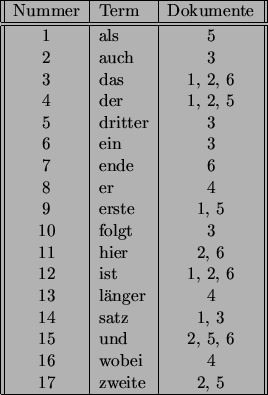
\includegraphics[scale=0.5]{../Abbildungen/index.png}
	\caption{Beispiel für einen invertierten Index}
\end{figure}